\chapter{Une application de test à grande envergure}

Mon stage débute le 8 avril. Une fois arrivé dans les locaux d'ORPALIS à Colomiers, Loïc et Cédric me présentent l'entreprise et ses objectifs.
C'est en comprenant l'envergure de GdPicture que je comprends la nécessité d'automatiser certains tests afin d'obtenir une visibilité en terme de fiabilité du SDK.

\section{Objectifs}

Loïc me présente une base de test contenant près d'un millier d'images de codes-barres classés par type.
Mon objectif principal est d'écrire une application qui, en utilisant GdPicture, va passer en revue chaque image et tenter d'y détecter un code-barres.
Il s'agira d'enregistrer les résultats des détections, afin d'émettre des rapports sur la quantité d'images lues et le nombre de codes-barres détectés.
L'idée est d'effectuer une analyse complète de la base de test à chaque nouvelle version du moteur de détection du SDK, afin de comparer les résultats ; il faudra donc envisager un mécanisme de comparaison des différents rapports entre eux.

Les tests sont une activité qui prend du temps et des ressources, c'est pour cela qu'une machine puissante tourne en permanence aux bureaux d'ORPALIS.
Cette machine contient un processeur capable d'effectuer plusieurs tâches en parallèle. Chaque tâche parallèle est exécutée sur ce que l'on appelle un fil d'exécution (en anglais, \og thread\fg ).
Ainsi, pour exploiter pleinement les performances d'une telle machine, il est nécessaire de concevoir son application pour qu'elle utilise plusieurs threads. On dit de cette application qu'elle est multi-threadée.

Il est bien entendu que la base de test dont je dispose n'est qu'un fragment de la vraie base de test qui contient, elle, bien plus d'images.
Il est impensable de ne traiter les images qu'une à une, c'est pourquoi Loïc me fournit un modèle d'application multi-threadée sur lequel je base mon développement.

\section{Développement}

Le développement de cette application a duré près d'un mois, du 8 avril au 3 mai.

\subsection{Le module de détection}

La première chose à réaliser est le module de détection des codes-barres. L'application doit être capable d'adapter la détection au code-barres et employer le bon algorithme pour pouvoir le tester.
Il existe quatre famille de codes-barres :

\begin{description}
 \item[1D] ils sont reconnaissables par leurs bandes verticales, ce sont les plus communs et il en existe plusieurs sortes.
 \item[DataMatrix] se sont des codes-barres en deux dimensions permettant de stocker jusqu'à 2335 caractères sur 1 cm\up{2}.
 \item[PDF417] des codes-barres en deux dimensions repérables notamment sur les billets d'avion.
 \item[QRcode] permet de stocker 4296 caractères alphanumériques, repérable aux carrés servant à la détection d'erreurs.
\end{description}

GdPicture possède une fonction de détection pour chacune de ces quatre familles. Dans le fichier de configuration, je peux définir quelle fonction utiliser pour un répertoire donné, ainsi toutes les images de ce répertoire seront analysées par cette seule fonction. Je peux sinon choisir d'utiliser les quatre fonctions. L'intérêt d'une telle démarche est que pour certaines images, je suis sûr qu'elles seront détectées par une fonction en particulier. Les résultats d'une détection PDF417 sur des QRcodes ne seraient pas significatifs, aussi ai-je intérêt à spécifier l'utilisation de la fonction de détection des QRcodes. Je pourrai donc observer l'évolution de la détection QRcode pour chaque image.\\
A l'inverse, il peut être utile de ne spécifier l'utilisation d'aucune fonction en particulier. Dans le cas d'image contenant des codes-barres de types différents, cela est primordial. Dans tous les cas, ces instructions doivent être écrites dans le fichier de configuration, et tout répertoire non référencé sera ignoré. Il est donc nécessaire de passer du temps à bien organiser le jeu de test et de configurer l'application en conséquence\footnote{Pour plus de détails, consulter l'annexe \ref{configFile}}.

\paragraph{}

La méthode de détection de GdPicture retourne une valeur qui indique si une erreur est survenue. Je n'ai pas eu à traiter de cas d'erreurs avec ces images dans la mesure ou il s'agit d'un jeu de test simple et éprouvé à plusieurs reprises.

GdPicture m'a tout de même donné du fil à retordre lorsque je me suis aperçu que lors d'une détection multi-threadée sur des QRcodes, les résultats variaient d'une passe à l'autre. La raison était que la fonction de détection retournait de manière imprévisible une erreur générique\footnote{Une erreur générique est le type d'erreur retourné lorsque l'on n'a pas pu identifier l'origine de l'erreur.}. La raison de cette erreur se situait à la fois dans GdPicture et dans mon application.\\
En effet, lors de l'exécution d'un programme sur plusieurs threads, la consommation de mémoire vive est proportionnelle au nombre de threads utilisés. Dans mon cas, chaque thread charge une image en mémoire, la traite, et effectue plusieurs autres opérations. Lorsque l'application se lance sur 4 threads, on ne constate aucun problème, mais lorsque le nombre de threads est augmenté à 16, 32 ou 64, la consommation de mémoire augmente rapidement. Ainsi on arrive à saturation et le système d'exploitation n'est plus en mesure d'accorder plus de mémoire à l'application. Pour éviter cette situation, le programme qui demande des accès en mémoire doit vérifier qu'assez d'espace est disponible pour lui or, une erreur dans GdPicture faisait que ce n'était pas le cas. Ainsi, la fonction de détection, essayant d'allouer de l'espace mémoire, se retrouve confrontée au problème de saturation et retourne une erreur générique, d'où les différences dans les résultats de détection, modulés au gré de la saturation mémoire.

Une fois la détection faite, je vérifie combien de codes-barres ont été détectés dans l'image. Si des codes-barres ont été détectés, je les compare avec le fichier témoin de l'image. Le fichier témoin contient la valeur du code-barre contenu dans l'image. Cette valeur pourra être obtenue par un autre moteur de détection. Si l'image contient plusieurs codes-barres, alors chaque valeur sera inscrite sur une ligne du fichier, sans ordre particulier\footnote{Le fichier témoin doit avoir le même nom que l'image à laquelle il est associé. Si le fichier est mal nommé ou manquant, l'image sera ignorée du test.}. Pour chaque image, je parcours donc le fichier témoin à la recherche de la valeur détectée. Si la valeur est trouvée, le code-barres est marqué comme détecté et correct. Si la valeur n'est pas trouvée, le code-barres est marqué comme détecté mais incorrect.

\begin{figure}
\begin{center}
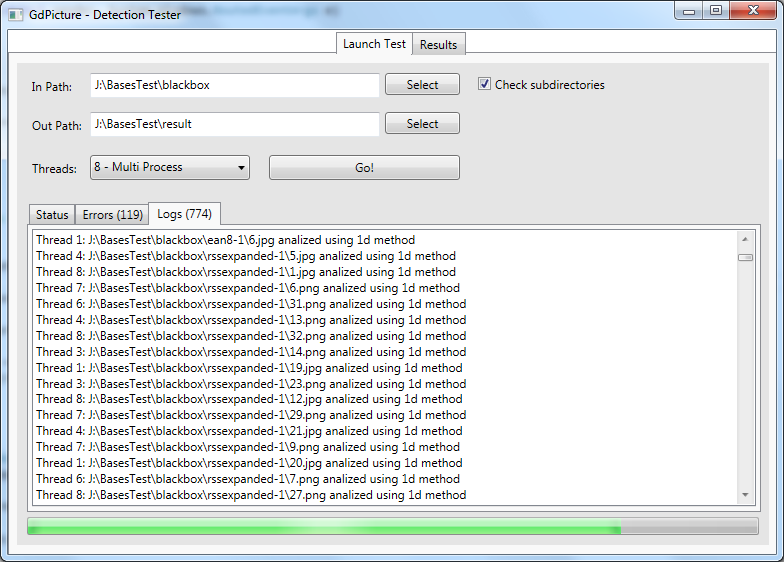
\includegraphics[scale=0.6]{images/projet1DetectionWindow.png}
\caption{Une détection en cours}
\end{center}
\end{figure}

\subsection{Création de rapports}

Chaque passage sur la base de tests va générer un rapport. L'un des objectifs de l'application est de pouvoir comparer plusieurs rapports. Le cas typique d'utilisation sera la réalisation d'un nouveau rapport à chaque nouvelle version du moteur de détection. Il est donc important de pouvoir stocker ces rapports afin de pouvoir les comparer au moment voulu. Le meilleur moyen est d'utiliser des fichiers.

Pour pouvoir structurer l'information dans un fichier, il faut utiliser une norme de notation. C'est à ça que servent les langages comme XML et ses dérivés. J'avais dans un premier temps commencé à utiliser XML mais très vite j'ai été limité par les contraintes de mise en forme du langage. Je me suis donc tourné vers un format plus récent : JSON. Historiquement dédié au web, JSON a l'avantage de disposer d'une syntaxe simple et souple.

J'ai pu trouver une bibliothèque .NET gérant la traduction en JSON\footnote{Disponible ici : http://james.newtonking.com/projects/json-net.aspx}. L'intérêt de cette bibliothèque est qu'elle permet de faire abstraction de la constitution d'un objet pour le traduire\footnote{On dit de cet objet qu'il est \og parsé \fg{} }. Il me suffit de donner un objet à une fonction de parsage pour qu'elle me renvoie le résultat en JSON. Il ne me reste donc qu'à écrire ce résultat dans le fichier.

En appliquant cette opération à toutes les images, on obtient donc un fichier contenant l'ensemble des informations de la détection pour toute la base de tests.

\subsection{Présentation des résultats}

A tout moment, il sera possible de comparer les rapports existants. Pour plus de commodité tous les rapports doivent être placés dans le même répertoire. Avec le chemin de ce répertoire, l'application doit être capable de retrouver les informations de chaque rapport et de les classer. Il est ensuite possible de choisir un rapport comme référence et d'afficher les différences de détection dans chaque rapport relativement à celui-ci. On étudie ici le taux de détection, c'est à dire le nombre de codes-barres corrects par rapport au nombre total.


\section{Bilan}

L'enjeu de cette application était de donner à ORPALIS un moyen de surveiller simplement les différences de détection entre les différentes versions du moteur. Une fois le jeu de test organisé et l'application configurée, il est très rapide de lancer une détection sur la base de test, d'enregistrer le rapport avec ceux existants et de comparer les résultats. La classification par type de détection, puis par fichier permet de donner un maximum d'informations tout en garantissant des résultats organisés et une analyse pertinente.

Ce projet aura été l'occasion de découvrir le langage C\#, l'environnement .NET et la spécification graphique WPF. L'utilisation des outils Microsoft assure la meilleure intégration de l'application dans Windows, permettant ainsi d'obtenir une application performante sans un gaspillage trop important de ressources. Le modèle d'application multithreadée de Loïc m'a permis de faire abstraction de cette contrainte dans la découverte de mon espace de travail. J'ai dû tout de même m'y confronter et construire mon application à l'intérieur. C'est en analysant le code source donné et en y greffant le mien que j'ai pu comprendre le fonctionnement du multi-threading en C\#.